

\section{Baseline calibration results {\color{LimeGreen} Laurence}}
\label{se:photometry_baseline}

We test the calibration bias and statistical uncertainties using the
baseline calibration method, which we recall, relies on the following
main ingredients: atmospheric attenuation is corrected using
the \emph{corrected skydip} opacity correction described in
Sect.~\ref{se:corrected-skydip}
and the telescope-driven beam impact is mitigated using the
\emph{baseline} scan selection described in
Sect.\ref{se:data_selection}.

The calibration bias is evaluated using a series of scans of MWC349
acquired during the N2R9, N2R12 and N2R14 campaigns. Namely, we use
the 72 scans that met the baseline selection criteria over the 109
available scans for MWC349.
Figure~\ref{fig:mwc349_obstau_corrected_skydip} shows the
bias for Array 1, Array 3, the combination of the $1~\rm{mm}$ arrays and
Array 2 as a function of the atmospheric transmission. This quantity
relates to the zenith opacity and the airmass as
$\exp \left( - \tau \cdot x \right) $.


\begin{figure}[ht!]
  \begin{center}
    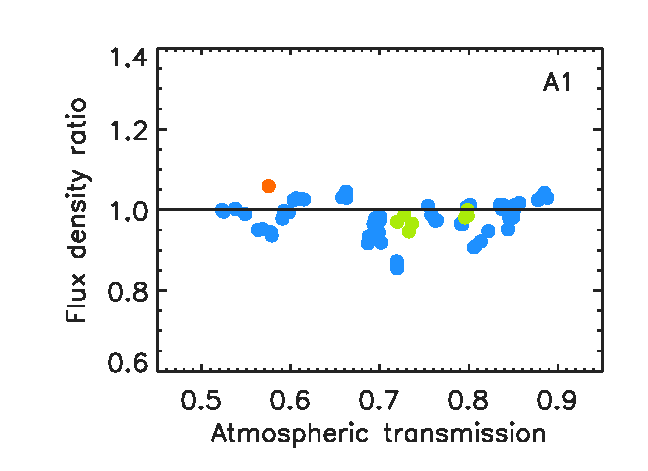
\includegraphics[clip=true, trim={0.9cm, 0, 0, 0.6cm},width=0.4\textwidth]{Figures/Calibration/plot_flux_density_ratio_MWC349_obstau_corrected_skydip_narrow_a1.pdf}
    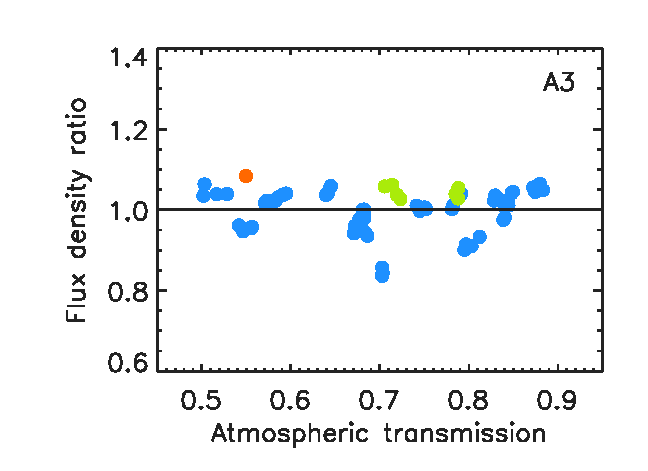
\includegraphics[clip=true, trim={0.9cm, 0, 0, 0.6cm},width=0.4\textwidth]{Figures/Calibration/plot_flux_density_ratio_MWC349_obstau_corrected_skydip_narrow_a3.pdf}
    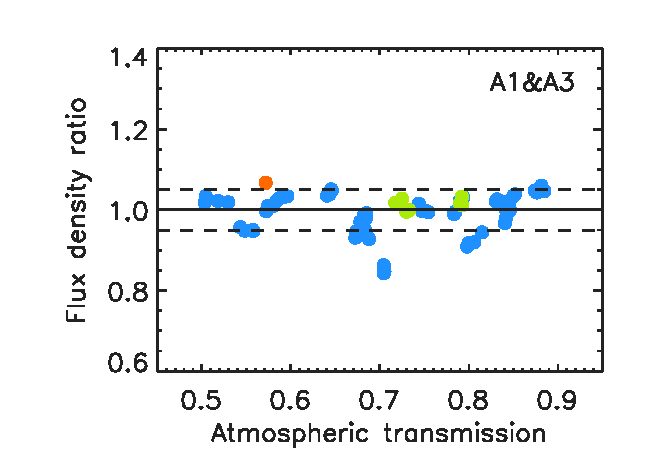
\includegraphics[clip=true, trim={0.9cm, 0, 0, 0.6cm},width=0.4\textwidth]{Figures/Calibration/plot_flux_density_ratio_MWC349_obstau_corrected_skydip_narrow_1mm.pdf}
    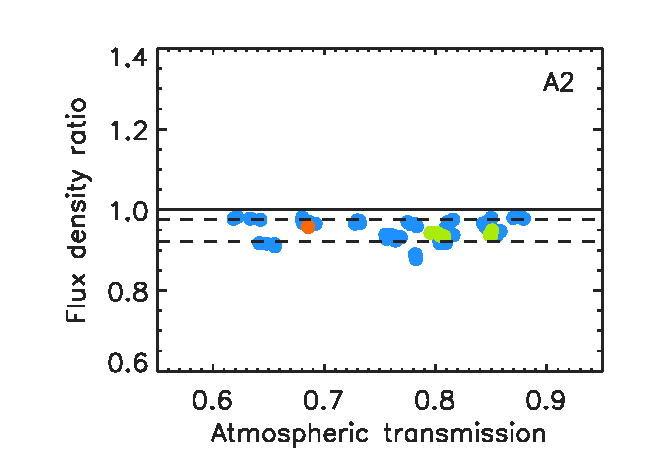
\includegraphics[clip=true, trim={0.9cm, 0, 0, 0.6cm},width=0.4\textwidth]{Figures/Calibration/plot_flux_density_ratio_MWC349_obstau_corrected_skydip_narrow_a2.pdf}
    \caption[Baseline calibration bias]{Baseline calibration
      bias. The measured-to-expected flux density ratio is shown as a
      function of the atmospheric transmission, defined as $\exp
      \left( - \tau \cdot x \right)$, using MWC349 scans acquired during N2R9 (blue),
      N2R12 (orange) and N2R14 (lime green) campaigns. Dashed lines
      show the flux density ratio $1 \sigma $ dispersion.}
    \label{fig:mwc349_obstau_corrected_skydip}
  \end{center}
\end{figure}

For the $1~\rm{mm}$ arrays and array combination, we find calibration
biases in agreement with unity within the statistical dispersion for
the three campaigns, whereas a $5\%$ lack of flux with respect to
expectations is observed at $2~\rm{mm}$, consistently for the three
campaigns. No sizable dependency of the calibration bias with the
atmospheric transmission is seen.

We further test the calibration
stability against atmospheric condition as described in
Sect.~\ref{se:photometry_criteria}. From a total of 487 scans
flux-selected sources acquired during N2R9, N2R12 and N2R14, 264 met
the baseline selection criteria and are used for testing stability.
The first panels of Fig.~\ref{fig:allbright_rms_corrected_skydip} show the
measured-to-median flux densities evaluated from these scans for Array
1, Array 3, the combination of Array $1\&3$ and Array 2 as a function of the
atmospheric transmission.

In addition, the statistical calibration uncertainties are
estimated using the standard deviation of the flux density ratios
using all the selected scans. We find uncertainties of $5.5\%$ for A1,
$6.1\%$ for A3, $5.7\%$ for the $1~\rm{mm}$ band and $2.9\%$ for A2.
These $1~\sigma$ statistical
errors are shown as the inner dashed lines from either sides of the
unity lines in Fig.~\ref{fig:allbright_rms_corrected_skydip}, while
$3\sigma$ errors are shown as the outer dashed lines.

No sizable dependency of the flux density ratio is seen within the
wide range of atmospheric transmission that have been tested, which goes
from 0.5 to 0.9. For most of the scans,
the flux density ratio is well within the $1~\sigma$ errors, whereas
some scans at atmospheric transmissions of about 0.7 show a mild lack
of flux density with respect to the median at a significance below
$3\sigma$.

We further investigated this lack of flux in the third row of
Fig.~\ref{fig:allbright_rms_corrected_skydip}. The flux density ratio
versus atmospheric transmission in the $1~\rm{mm}$ and $2~\rm{mm}$
bands are shown color-coded as a function of the observation date. The
scans affected by the lack of flux have all been observed 
either between 12:00 and 14:00 UT or between 8:00 and 9:00 UT hours,
that are close to the observation date cut thresholds of the baseline
selection (see Sect.~\ref{se:data_selection}). These scans are likely
to be impacted by the telescope-driven beam broadening or by the
sunrise focus drift respectivelly.

We evaluate the calibration
uncertainty improvement that would result from a more restrictive
selection on the observation date. The last row of
Fig.~\ref{fig:allbright_rms_corrected_skydip} shows the flux density
ratio distribution at 1 and $2~\rm{mm}$. These consist in bulk Gaussian
distributions, which correspond to the nightly observations and large
distribution queues toward the low flux density ratio, due to morning
observations. Gaussian fits of these distributions mainly capture the
Gaussian bulk and are thus indicative of the uncertainty improvement
from narrower observation date windows. We find that restricting the
used observation dates to the 10 more stable hours (from $22:00$ to
$08:00$ UT) would result in improving the calibration uncertainties of
about $60\%$ at $1~\rm{mm}$ and $40\%$ at $2~\rm{mm}$. The baseline
selection, which i) retains 16 hours of observation time a day and ii)
results in calibration uncertainties that meet the requirement for a
millimetric ground-based instrument, constitutes an advantageous
tradeoff.  



\begin{figure}[ht!]
  \begin{center}
    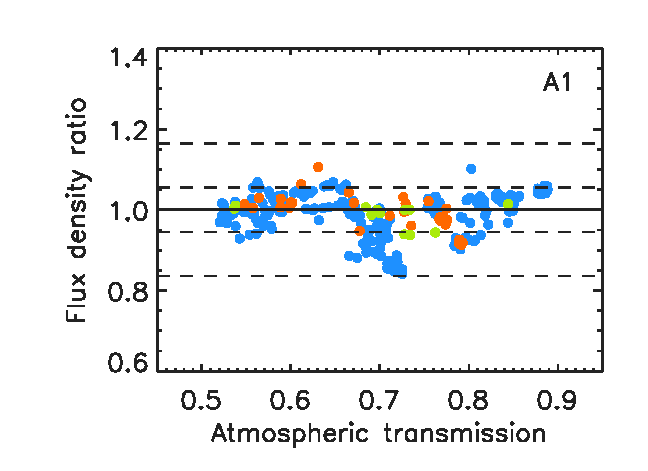
\includegraphics[clip=true, trim={0.9cm, 0.2cm, 0, 0.6cm}, width=0.4\textwidth]{Figures/Calibration/plot_flux_density_ratio_obstau_allbright_corrected_skydip_narrow_a1.pdf}
    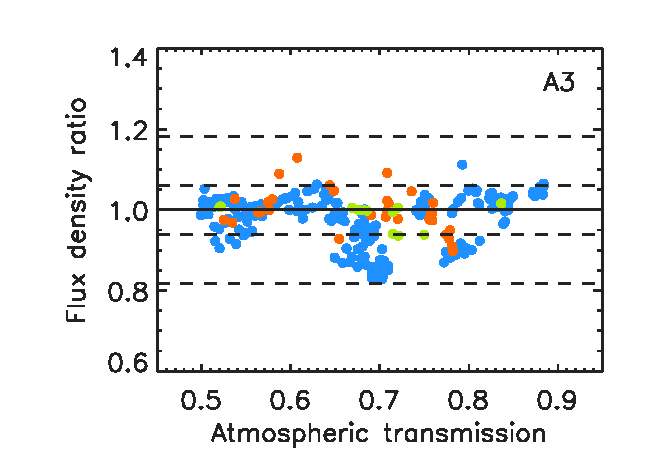
\includegraphics[clip=true, trim={0.9cm, 0.2cm, 0, 0.6cm},width=0.4\textwidth]{Figures/Calibration/plot_flux_density_ratio_obstau_allbright_corrected_skydip_narrow_a3.pdf}
    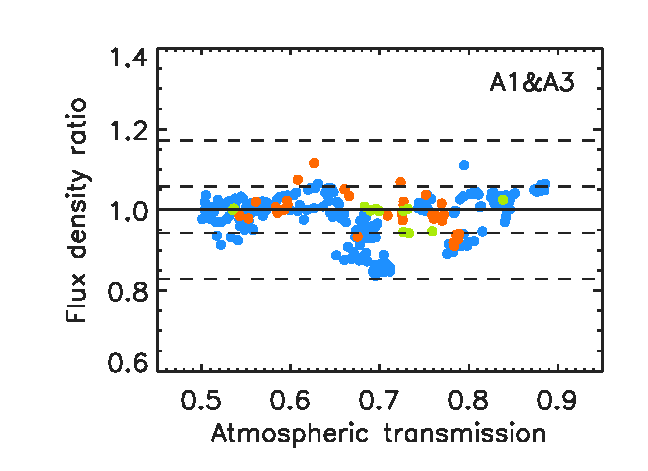
\includegraphics[clip=true, trim={0.9cm, 0.2cm, 0, 0.6cm},width=0.4\textwidth]{Figures/Calibration/plot_flux_density_ratio_obstau_allbright_corrected_skydip_narrow_1mm.pdf}
    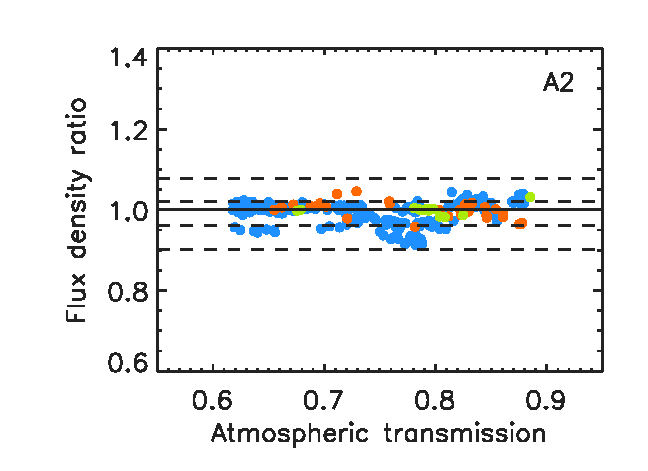
\includegraphics[clip=true, trim={0.9cm, 0.2cm, 0, 0.6cm},width=0.4\textwidth]{Figures/Calibration/plot_flux_density_ratio_obstau_allbright_corrected_skydip_narrow_a2.pdf}
    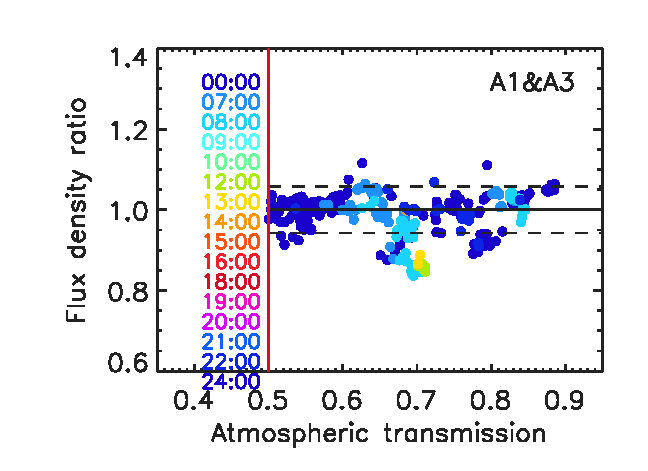
\includegraphics[clip=true, trim={0.9cm, 0.2cm, 0, 0.6cm},width=0.4\textwidth]{Figures/Calibration/plot_flux_density_ratio_obstau_allbright_obsdate_corrected_skydip_narrow_1mm.pdf}
    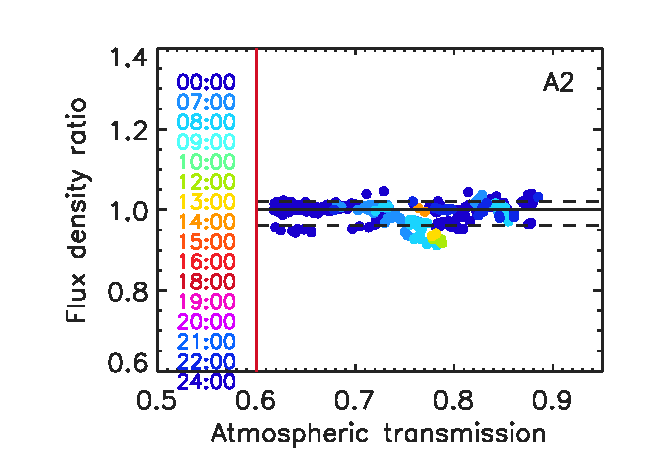
\includegraphics[clip=true, trim={0.9cm, 0.2cm, 0, 0.6cm},width=0.4\textwidth]{Figures/Calibration/plot_flux_density_ratio_obstau_allbright_obsdate_corrected_skydip_narrow_a2.pdf}
    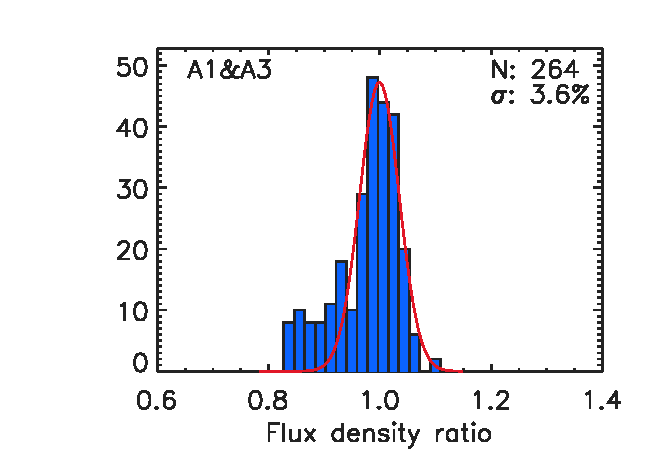
\includegraphics[clip=true, trim={0.9cm, 0.2cm, 0, 0.6cm},width=0.4\textwidth]{Figures/Calibration/plot_histo_flux_density_ratio_obstau_allbright_corrected_skydip_narrow_1mm.pdf}
    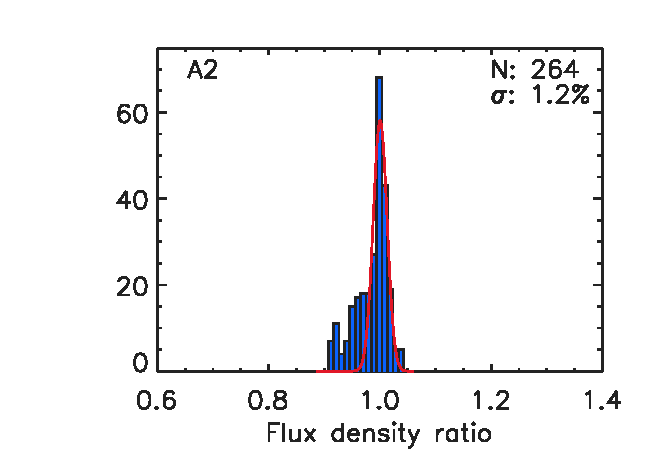
\includegraphics[clip=true, trim={0.9cm, 0.2cm, 0, 0.6cm},width=0.4\textwidth]{Figures/Calibration/plot_histo_flux_density_ratio_obstau_allbright_corrected_skydip_narrow_a2.pdf}  
    \caption[Baseline calibration rms error estimate]{Baseline
      calibration uncertainties. The four first panels shows the
      measured-to-median flux density ratio of bright sources vs
      atmospheric transmission using the baseline calibration for
      Array 1 (A1), Array 3 (A3), the combination of A1$\&$A3 and
      A2. Blue points are N2R9 scans, orange points N2R12 and lime
      green points N2R14. The dashed lines from either sides of the
      unity-ratio line
      show the $1\sigma$ (inner lines) and $3\sigma$ (outer lines) errors.
      The third row panels are copies of the 'A1$\&$A3' and the
      'A2' panels color-coded from the UT observation time of the
      scans. Lower flux ratio datapoints correspond to
      scans acquired after 8:00 UT hours. Flux density ratio
      distributions for A1$\&$A3 and A2 are plotted in the fourth row
      panels. The Gaussian fits of this distribution, plotted in red,
      mainly capture the
      night-time observation scans%Their widths are sizably smaller
      %than the rms error evaluated from all the scans
      , indicating the
      impact of scans acquired after 8:00 UT on the calibration
      uncertainties.}
    \label{fig:allbright_rms_corrected_skydip}
  \end{center}
\end{figure}

%  BASELINE RESULTS
%%%%%%%%%%%%%%%%%%%%%%%%%%%%%%%%%%%%%%%%%%%%%%%%%%%%%%%%%%%%%%%%%%
\begin{table}[th]
\begin{center}
\begin{tabular}{|c|l|c|c|c|c|}
  \hline
  \multicolumn{2}{|c|}{}  &  \multicolumn{4}{|c|}{Datasets}  \\\cline{3-6}
  \multicolumn{2}{|c|}{Characteristics} &  N2R9  & N2R12   &  N2R14 &  Combined \\
  \hline\hline
  Bias &  $\#$ total    &  68    &  14     &   27     &    109    \\
       &  $\#$ selected &  64    &   1     &   7      &     72    \\
       &  A1            &  0.99  &  1.06   &   0.98   &   0.98    \\
       &  A3            &  1.01  &  1.08   &   1.04   &   1.00    \\
       &  1mm           &  1.00  &  1.07   &   1.01   &   0.99    \\
       &  2mm           &  0.95  &  0.96   &   0.94   &   0.95    \\
  \hline
  \multicolumn{6}{|l|}{using color corrections as of Table A.1}  \\
  \hline
  Bias &  $\#$ total    &  68    &  14     &   27     &    109    \\
       &  $\#$ selected &  64    &   1     &   7      &     72    \\
       &  A1            &  0.95  &  1.03   &   0.94   &   0.95    \\
       &  A3            &  0.99  &  1.07   &   1.00   &   1.00    \\
       &  1mm           &  0.97  &  1.05   &   0.97   &   0.98    \\
       &  2mm           &  0.95  &  0.95   &   0.93   &   0.95    \\
  \hline
  Rms  &  $\#$ total    &  303   &  72     &   112    &    487   \\
       &  $\#$ selected &  219   &  33     &    12    &    264   \\
       &  A1            &  5.7   &  4.6    &   2.9    &    5.5   \\
       &  A3            &  6.2   &  5.7    &   2.4    &    6.0   \\
       &  1mm           &  5.9   &  5.0    &   2.5    &    5.7   \\
       &  2mm           &  3.2   &  2.1    &   1.1    &    3.0   \\  
\hline\hline
\end{tabular}
\caption[Baseline calibration results]{Baseline calibration results:
  photometry accuracy and uncertainties. The first row gives the calibration
  bias -- defined as the measured-to-expected flux density ratio --
  and the second row the calibration rms error -- defined as the
  standard deviation of the measured-to-median flux density of bright
  sources using observations during N2R9, N2R12, N2R14 and the
  combination of the three campaigns. }
\label{tab:baseline-photometry}
\end{center}
\end{table}


As a summary, the baseline calibration results in flux densities in
agreement with expectations for MWC349 at $1~\rm{mm}$ and $5\%$ below
expectations for MWC349 at $2~\rm{mm}$. This bias, which has a low
significance with respect to the absolute calibration precision of
both NIKA2 ($5\%$) and PdB, will be further investigated by using other
calibration methods in Sect.~\ref{se:photometry_others}. Moreover, the
photometry is stable against the atmospheric condition within
uncertainties over a wide range of opacities. The calibration
statistical errors are about $6\%$ at $1~\rm{mm}$ and $3\%$ at
$2~\rm{mm}$. All results for the baseline calibration are gathered in
Table~\ref{tab:baseline-photometry}.


